%Starting.
\pgfdeclarelayer{frontmost}
\pgfdeclarelayer{colnameslayer}
\pgfsetlayers{main,frontmost,colnameslayer}
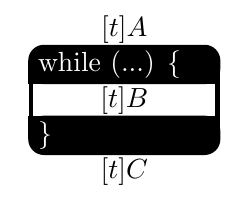
\begin{tikzpicture}[x=1mm,y=1mm,scale=1.]
% State has been set.
\begin{pgfonlayer}{frontmost}
\draw [black] (13.5,-3.) node{\smash{$\ml[t]{A}$}};
\end{pgfonlayer}
\draw [line width = 0.6mm, black] (1.65,-10.) -- (1.65,-9.);
\draw [line width = 0.6mm, black] (25.35,-10.) -- (25.35,-9.);
\fill[fill=black, rounded corners=2.mm] (1.3,-9.) rectangle (25.7,-4.);
\fill[fill=black] (1.3,-9.) rectangle (25.7,-6.5);
\draw [white] (1.3,-6.5) node[anchor=west]{\code{while (...) \{}};
\draw [line width = 0.6mm, black] (1.65,-13.) -- (1.65,-9.);
\draw [line width = 0.6mm, black] (25.35,-13.) -- (25.35,-9.);
\begin{pgfonlayer}{frontmost}
\draw [black] (13.5,-12.) node{\smash{$\ml[t]{B}$}};
\end{pgfonlayer}
\draw [line width = 0.6mm, black] (1.65,-13.) -- (1.65,-12.);
\draw [line width = 0.6mm, black] (25.35,-13.) -- (25.35,-12.);
\fill[fill=black, rounded corners=2.mm] (1.3,-18.) rectangle (25.7,-13.);
\fill[fill=black] (1.3,-15.5) rectangle (25.7,-13.);
\draw [white] (1.3,-15.5) node[anchor=west]{\code{\}}};
\begin{pgfonlayer}{frontmost}
\draw [black] (13.5,-21.) node{\smash{$\ml[t]{C}$}};
\end{pgfonlayer}
\end{tikzpicture}
%Finished.
